\section{Veränderungen}
\subsection{Klassendiagramm}
Im Folgenden wird anhand des aktualisierten Klassendiagramms gezeigt, was sich zum Entwurf verändert hat.

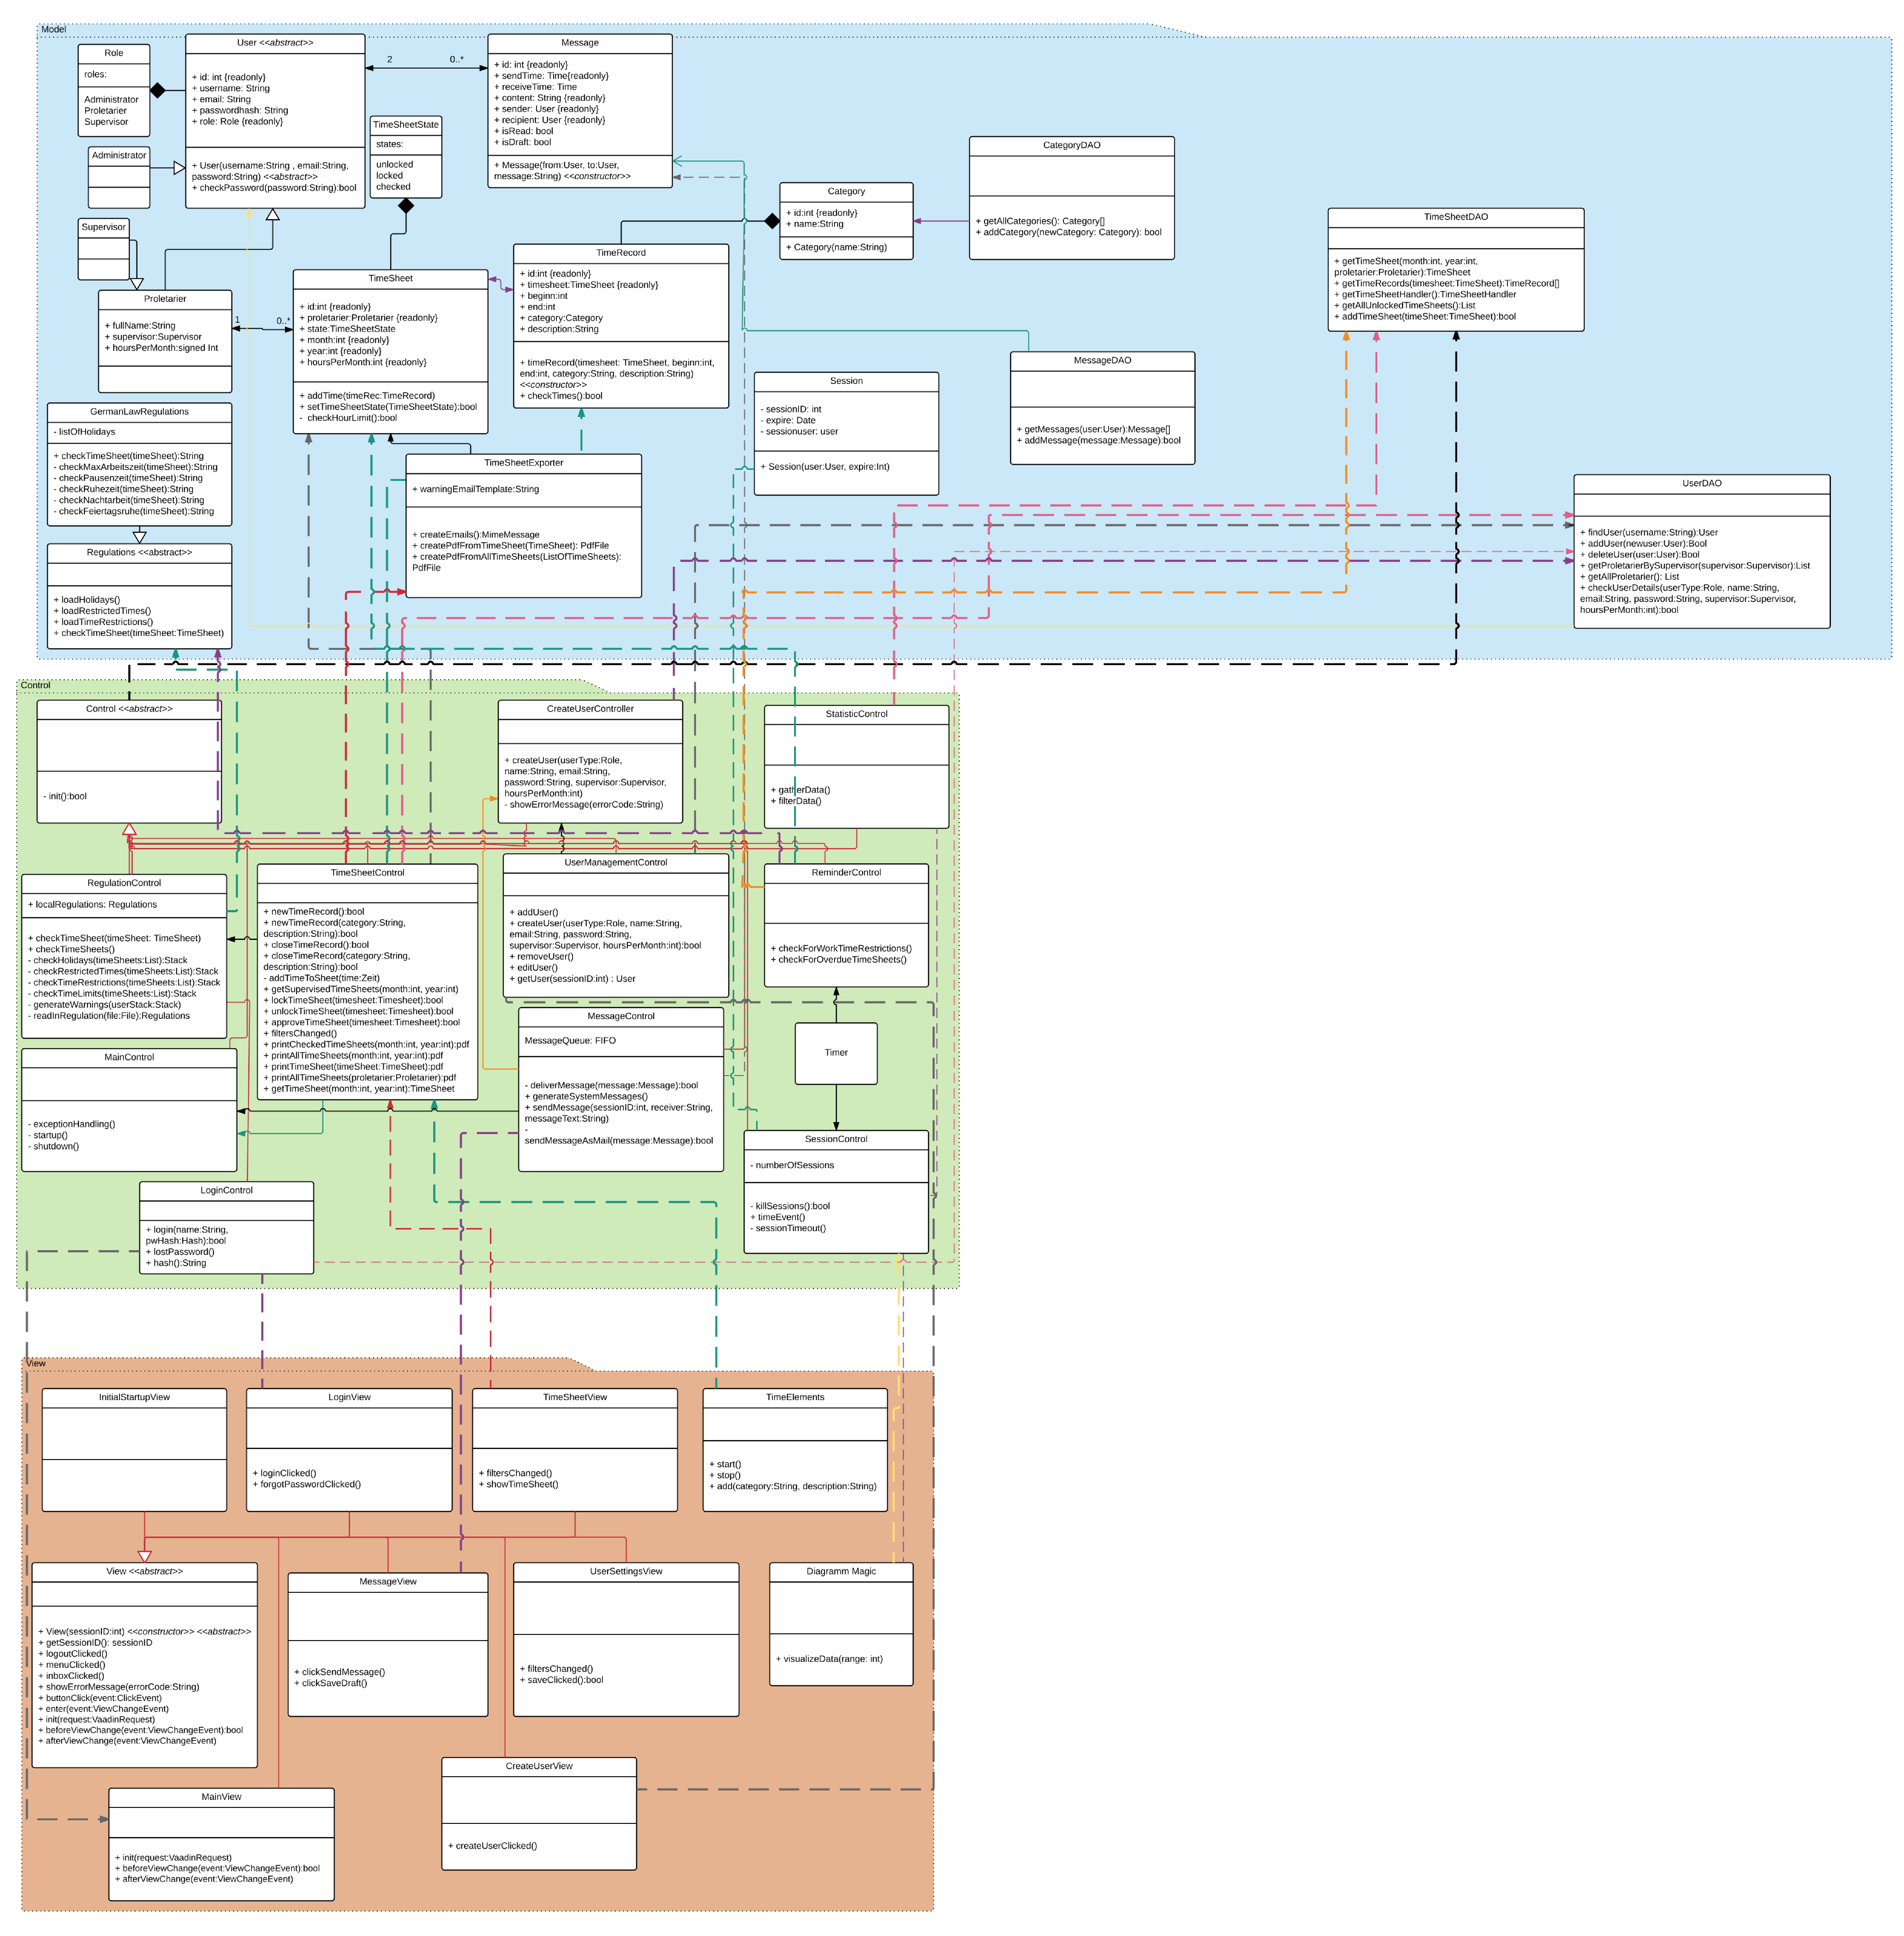
\includegraphics{Class-Diagramm_alt.pdf}
In der view haben sich folgenden Änderungen ergeben:
\VerbatimInput{view-diff}

Die meisten Änderungen in der \emph{View} sind durch Vaadin entstanden. 
Im speziellen mussten Methoden und Attribute angepasst oder hinzugefügt werden, 
damit \emph{Vaadin} funktioniert.
Es wurden auch drei neue Sichten hinzugefügt, \emph{AdminView}, \emph{SupervisorView} und \emph{TimeRecordView}, 
dafür wurde auch das Packet \emph{view.forms} erstellt.
Die abstrakte \emph{View} wurde gelöscht, da mit \emph{Vaadin} das gewünschte Entwurfsmuster 
ohne weitere Aufwendungen nicht umsetzbar war.
Die \emph{MessageView} wurde entfernt aufgrund einer Änderung der Anforderungen an das Projekt.

In der conrtol haben sich folgende Änderungen ergeben:
\VerbatimInput{control-diff}

Wie auch zuerst in der \emph{View} angedacht, wurde auch in der \emph{Control} die abstrakte \emph{Control} Klasse 
nicht wie beabsichtigt angewendet werden.
Es wurden zwei neue Klassen erstellt, welche für den \emph{Scheduler} benötigt werden. 
Die Klasse \emph{Timer} wurde zu \emph{SchedulerHandler} umbenannt, damit der Name besser zur Funktionalität passt.
Die Methoden aus der \emph{ReminderControl} wurden in das \emph{Model} verschoben.
Weitere Methoden mussten unter anderem zur \emph{UserManagementControl} und \emph{TimeSheetControl} hinzugefügt werden, 
um andere Funktionalitäten und Änderungen im \emph{Backend} korrekt zu unterstützen.

Im model haben sich folgende Änderungen ergeben: %TODO tex syntax
\VerbatimInput{model-diff}

%text


Daraus ergibt sich das aktualisierte Klassendiagramm:

%neues Klassendiagramm

\subsection{Sequenzen}
Die Sequenzdiagramme aus dem Entwurfen haben sich wie folgt verändert:
\subsubsection{Login Sequenz}

\begin{figure}
  \centering
    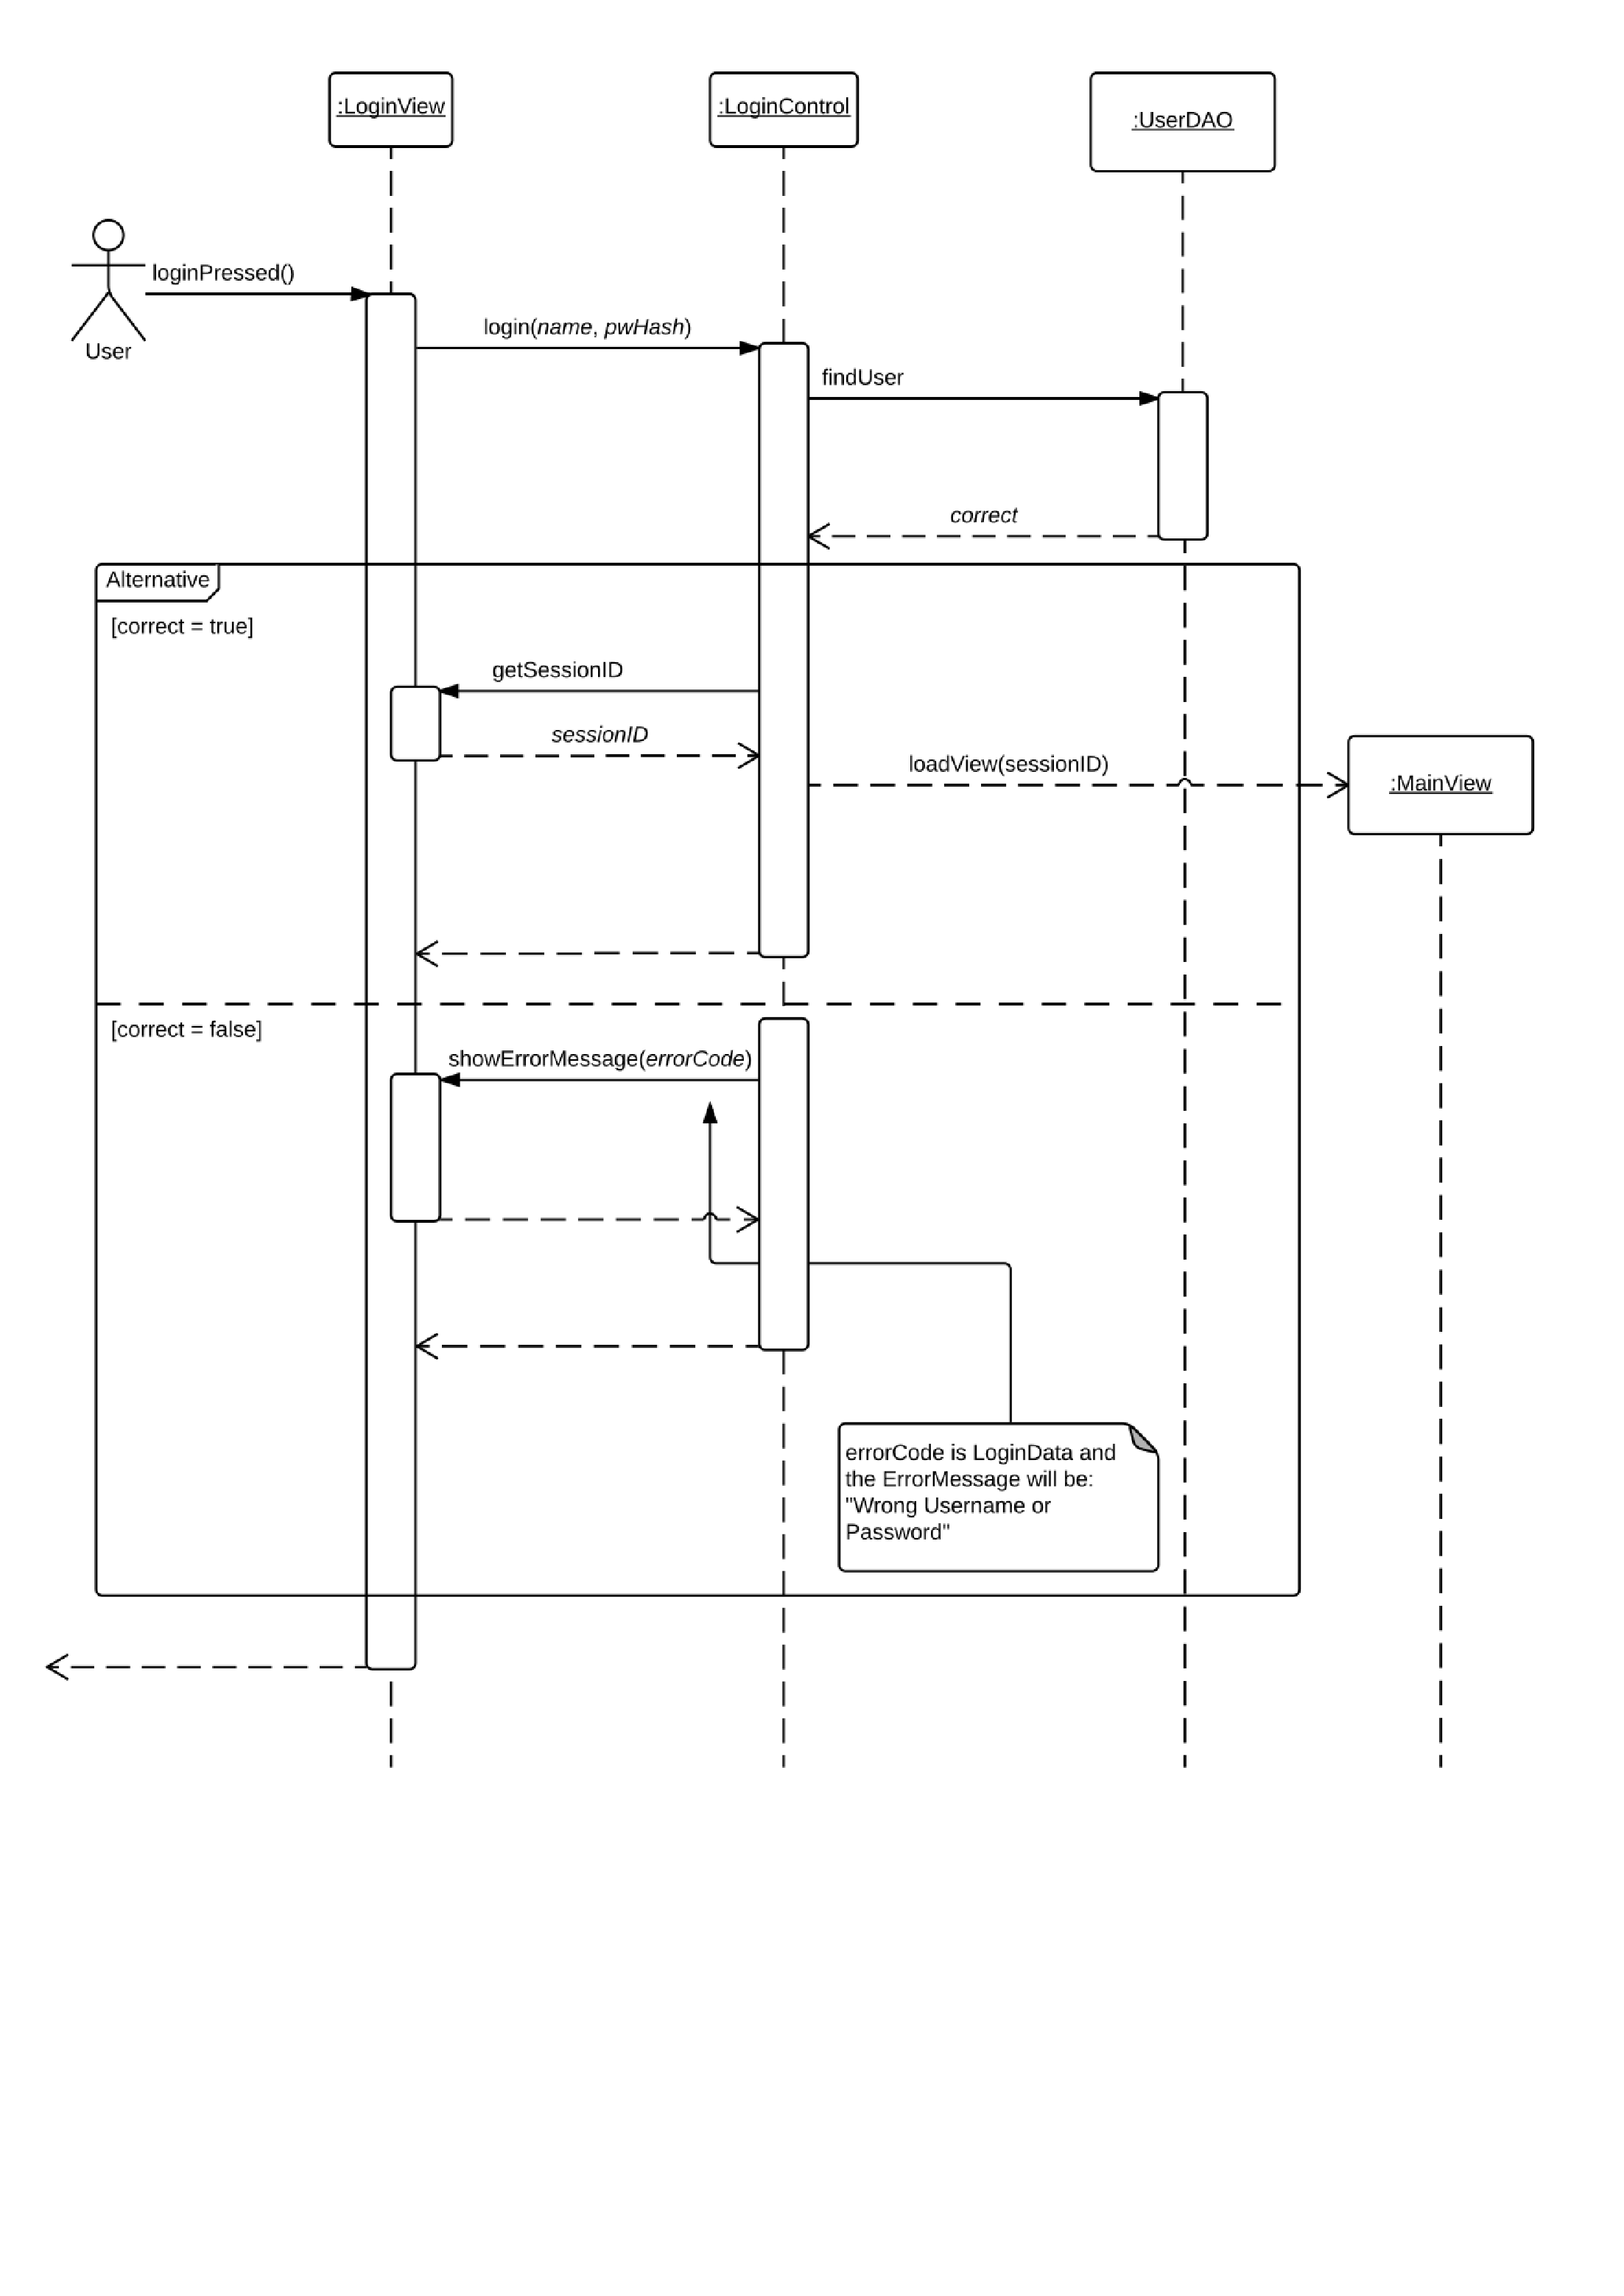
\includegraphics[width=\linewidth]{Login-Sequenz.pdf}
   \caption{Alte Login Sequenz}
\end{figure}

\paragraph{Veränderungen}
\begin{itemize}
    \item Login wurde um die Funktion \emph{remember me} erweitert.
    \item Die Authentifizierung wurde in einklang mit dem Shiro Framework gestaltet:
    \begin{itemize}
        \item Zum Login wird ein token aus Passwort und Username genutzt.
        \item Durch das Token wird der Nutzer ermittelt und dessen Authentifizierungsdaten(Password, ...) geholt.
        \item Diese werden mittels einen speziellen Hash vergleicher mit dem angegebenen Token verglichen.
    \end{itemize}
    \item Laden der View wurde durch Vaadins \emph{navigateTo} ersetzt.
\end{itemize}

\begin{figure}
  \centering
    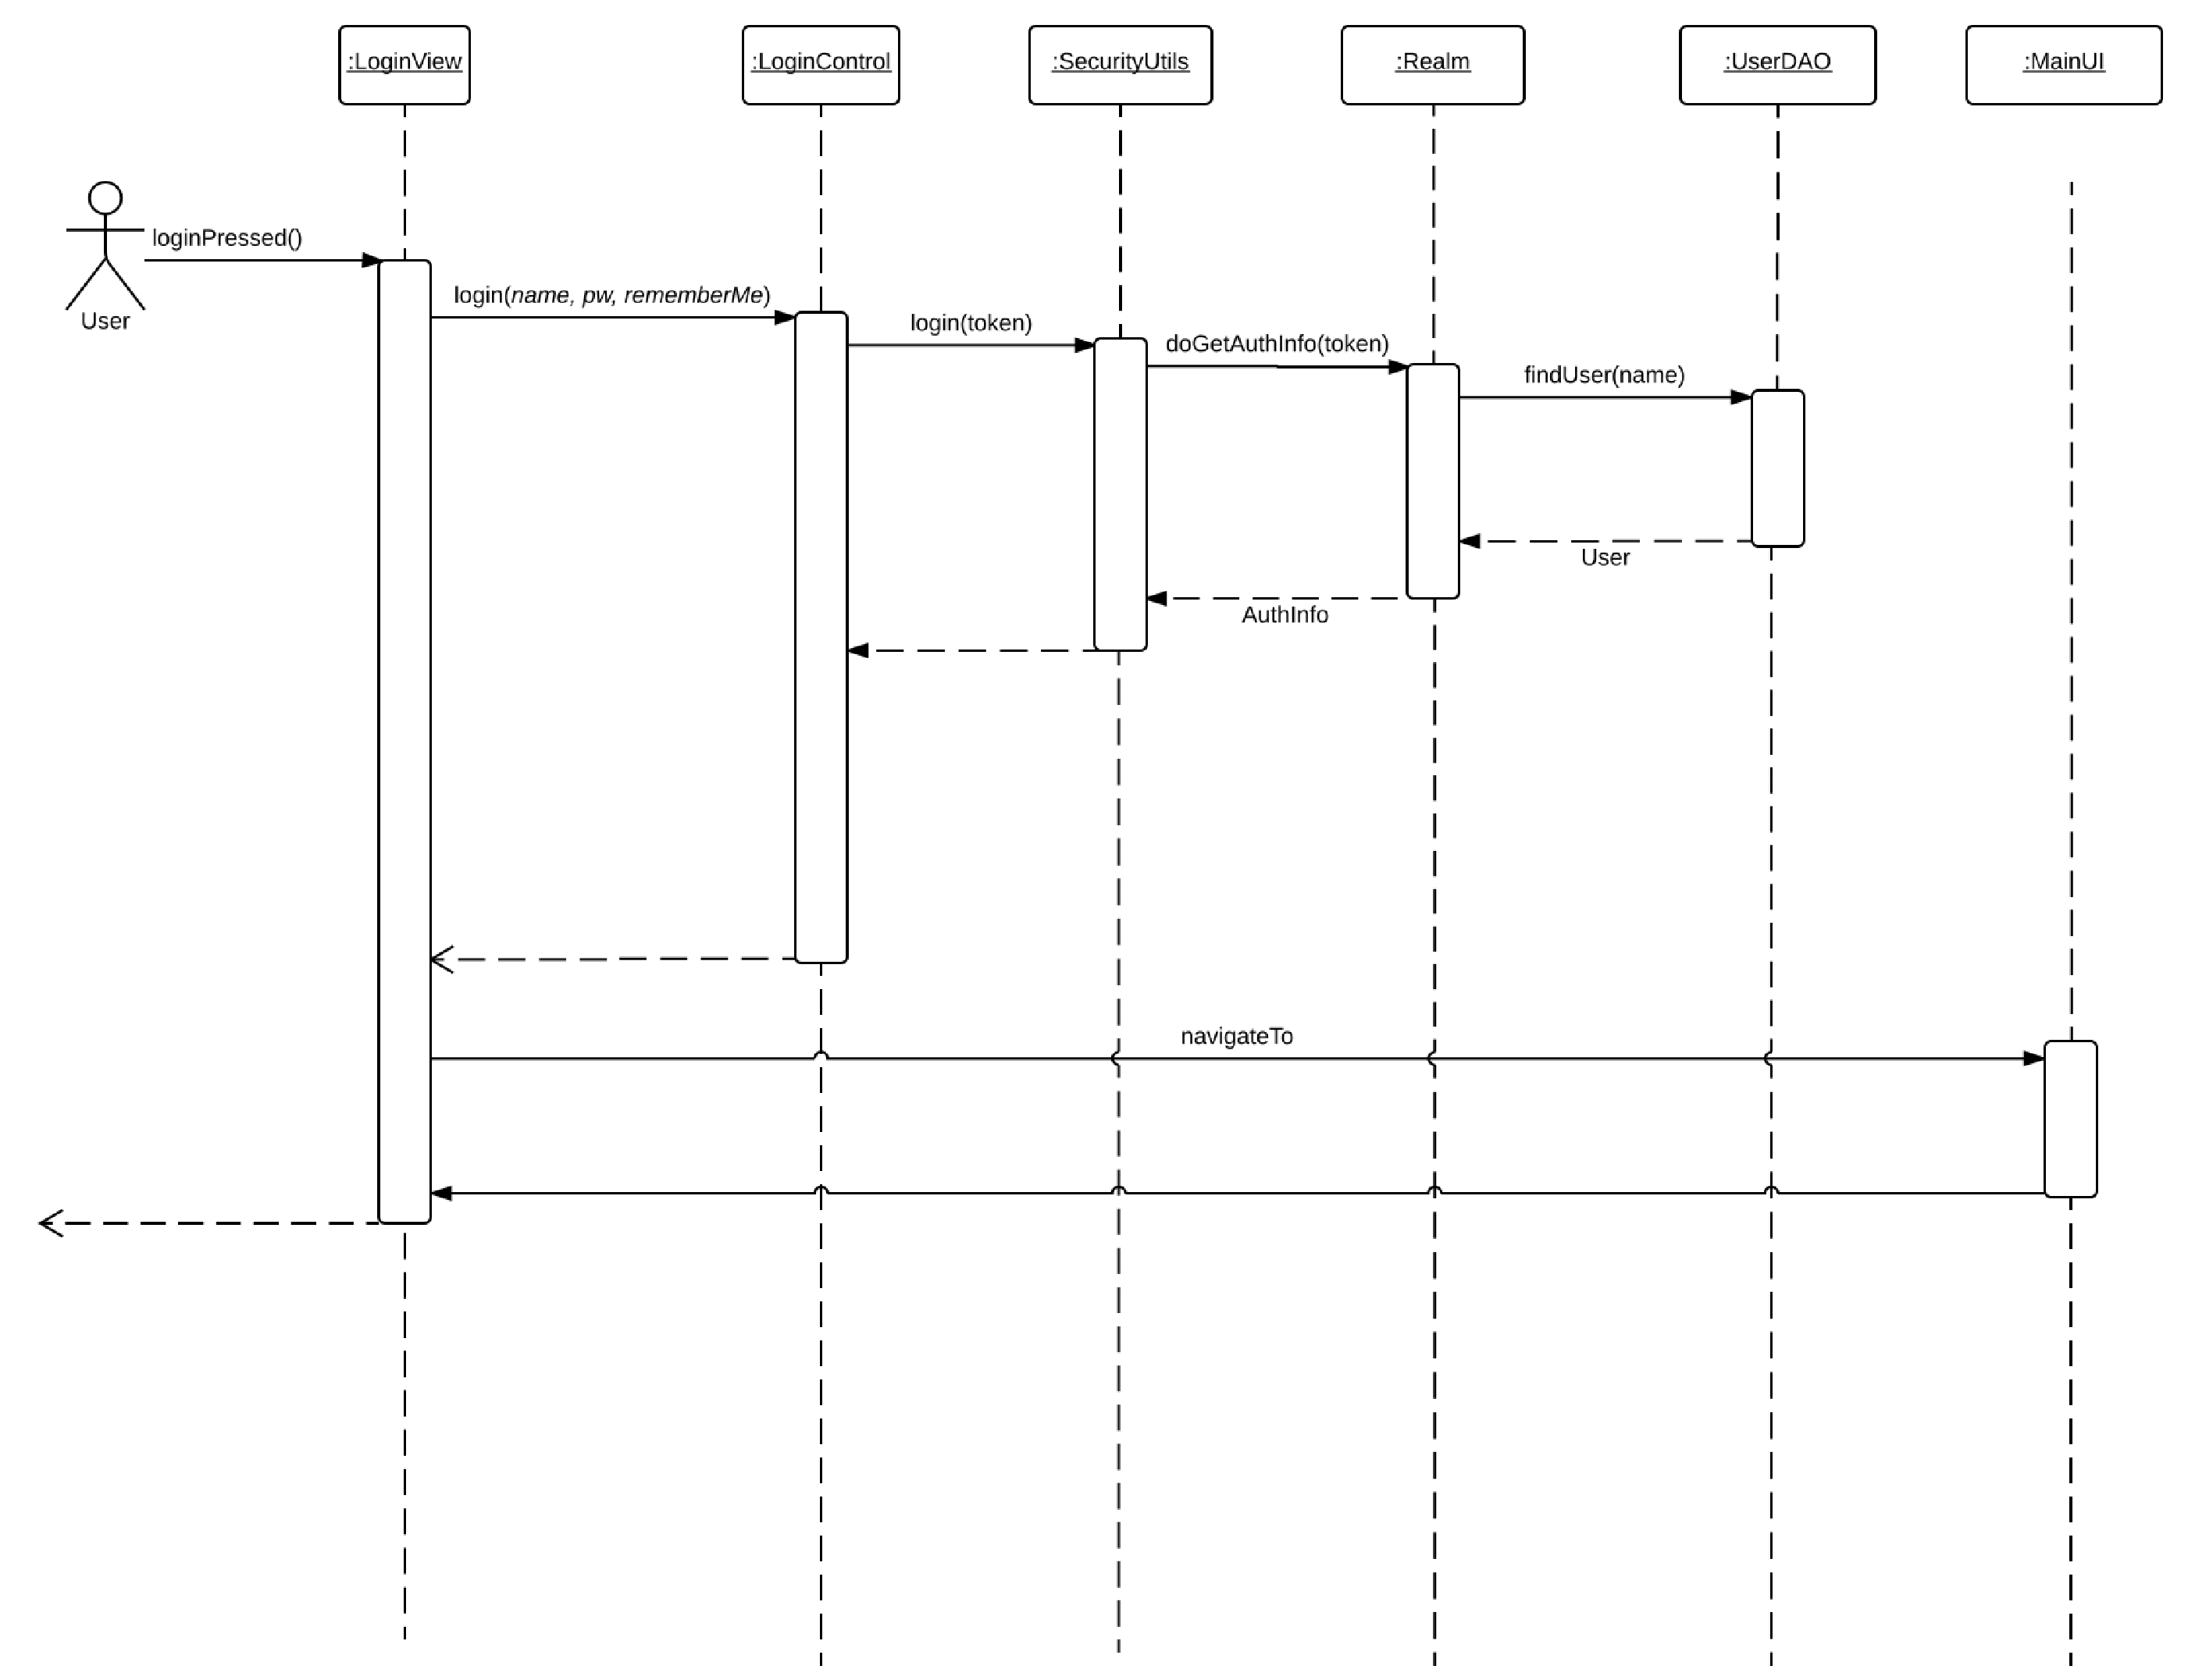
\includegraphics[width=\linewidth]{Login-Sequenz-new.pdf}
   \caption{Neue Login Sequenz}
\end{figure}

\subsection{Account erstellungs Sequenz}

\begin{figure}
  \centering
    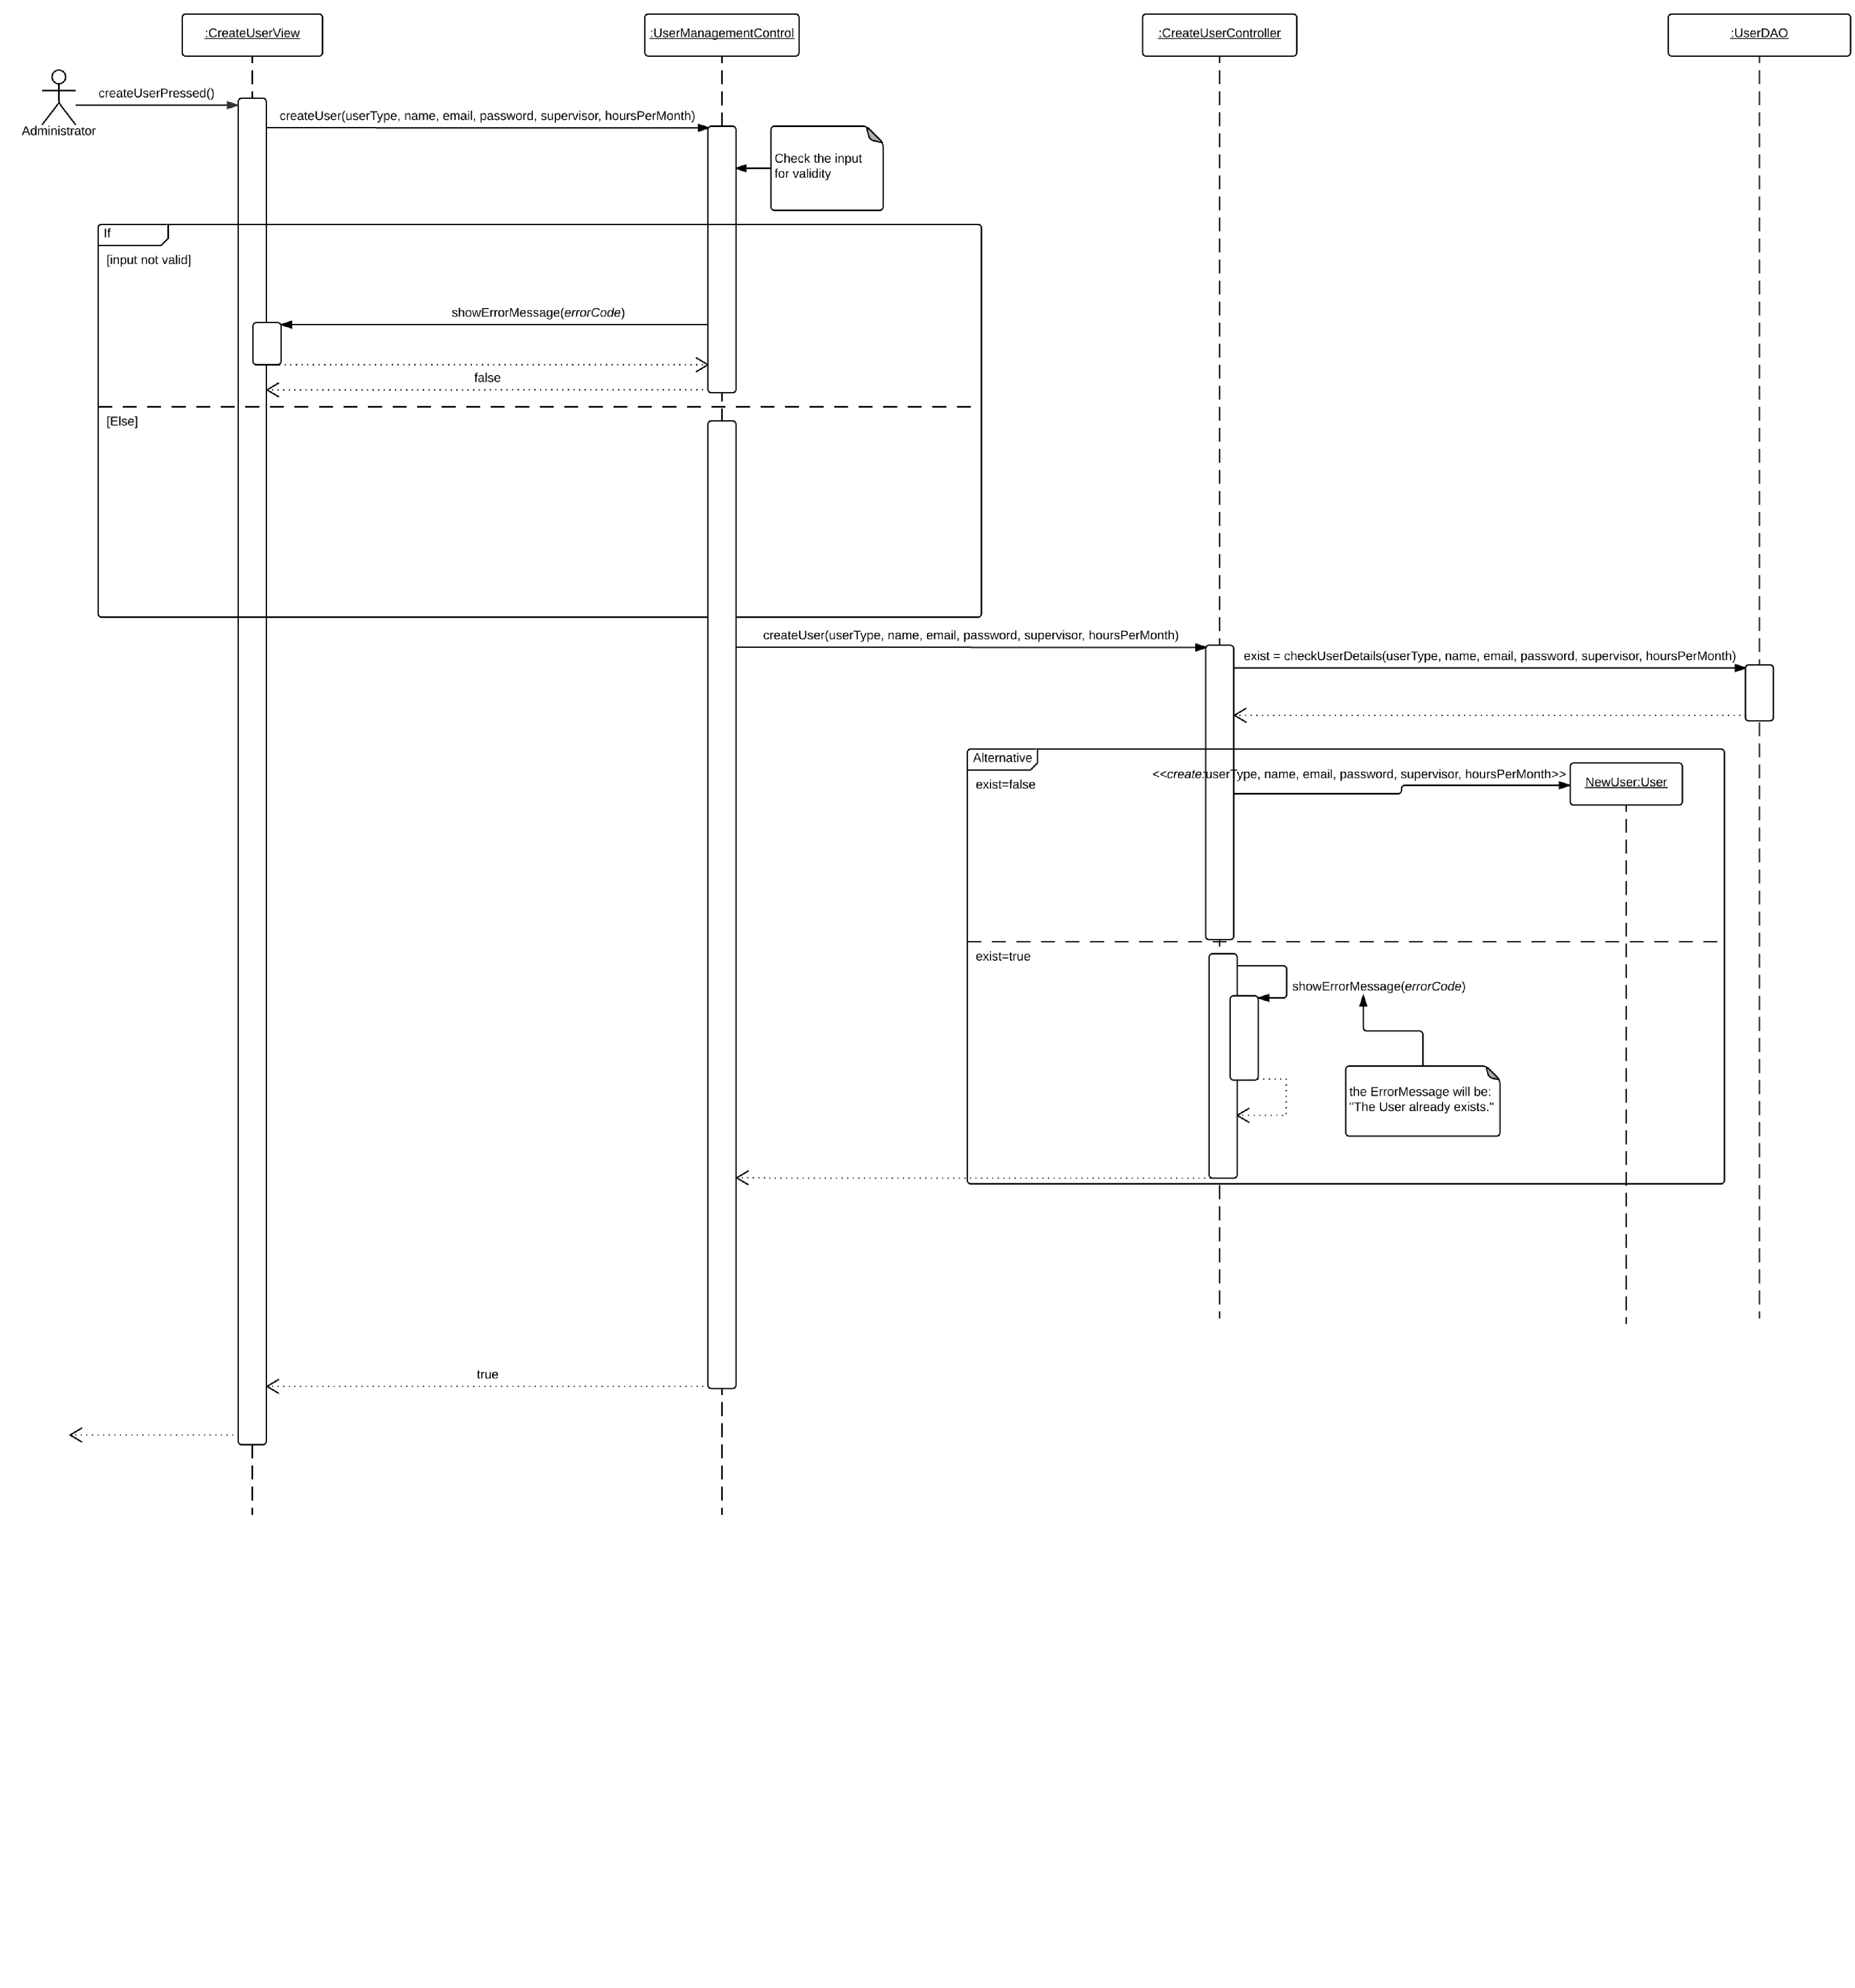
\includegraphics[width=\linewidth]{Create-user-account.pdf}
   \caption{alte Benutzererstellungssequenz}
\end{figure}

\paragraph{Veränderungen}
\begin{itemize}
    \item Der Ablauf wurde vereinfacht. Es wird nurnoch die CreateUserControl Klasse angespochen.
    \item Überprüfungen wurden durch eine verbesserte klarere interne Exception Struktur vereinfacht.
\end{itemize}

\begin{figure}
  \centering
    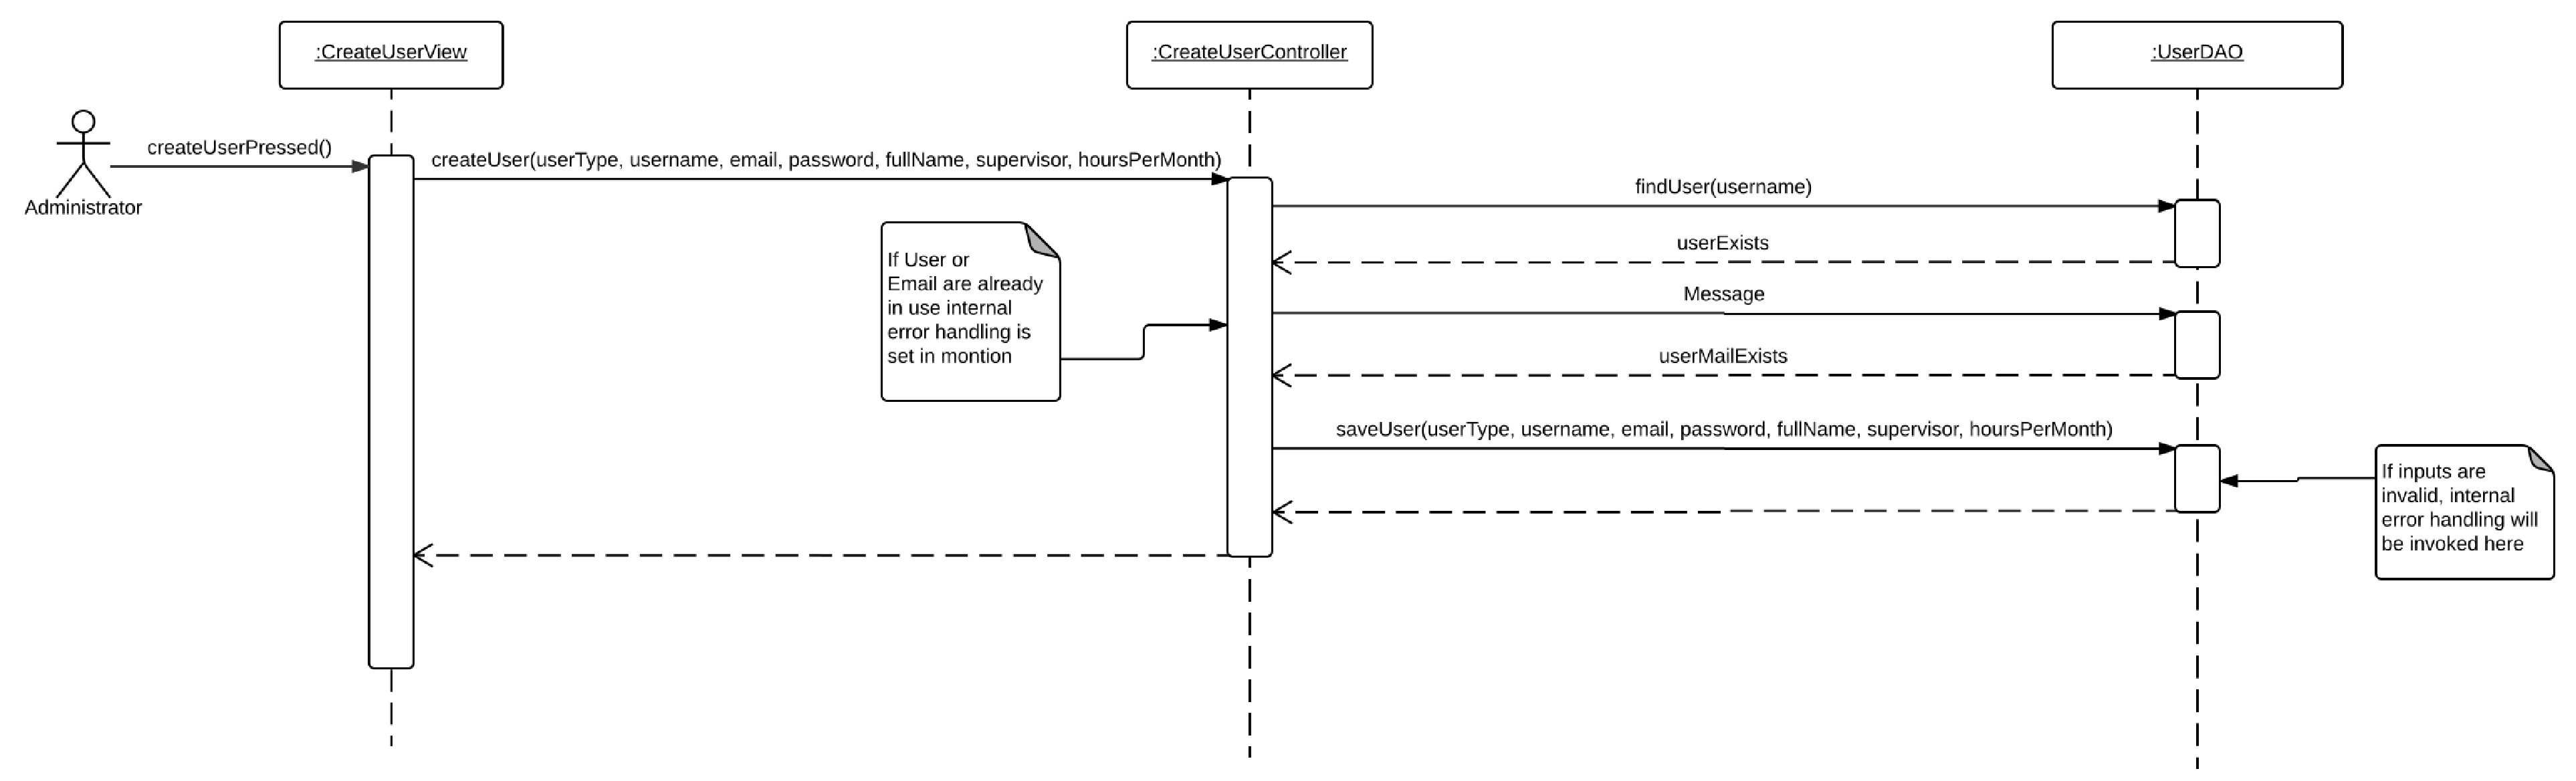
\includegraphics[width=\linewidth]{Create-user-account-new.pdf}
   \caption{Neue Benutzererstellungssequenz}
\end{figure}

\subsection{Neue Zeiterfassung - Sequenz}

\begin{figure}
  \centering
    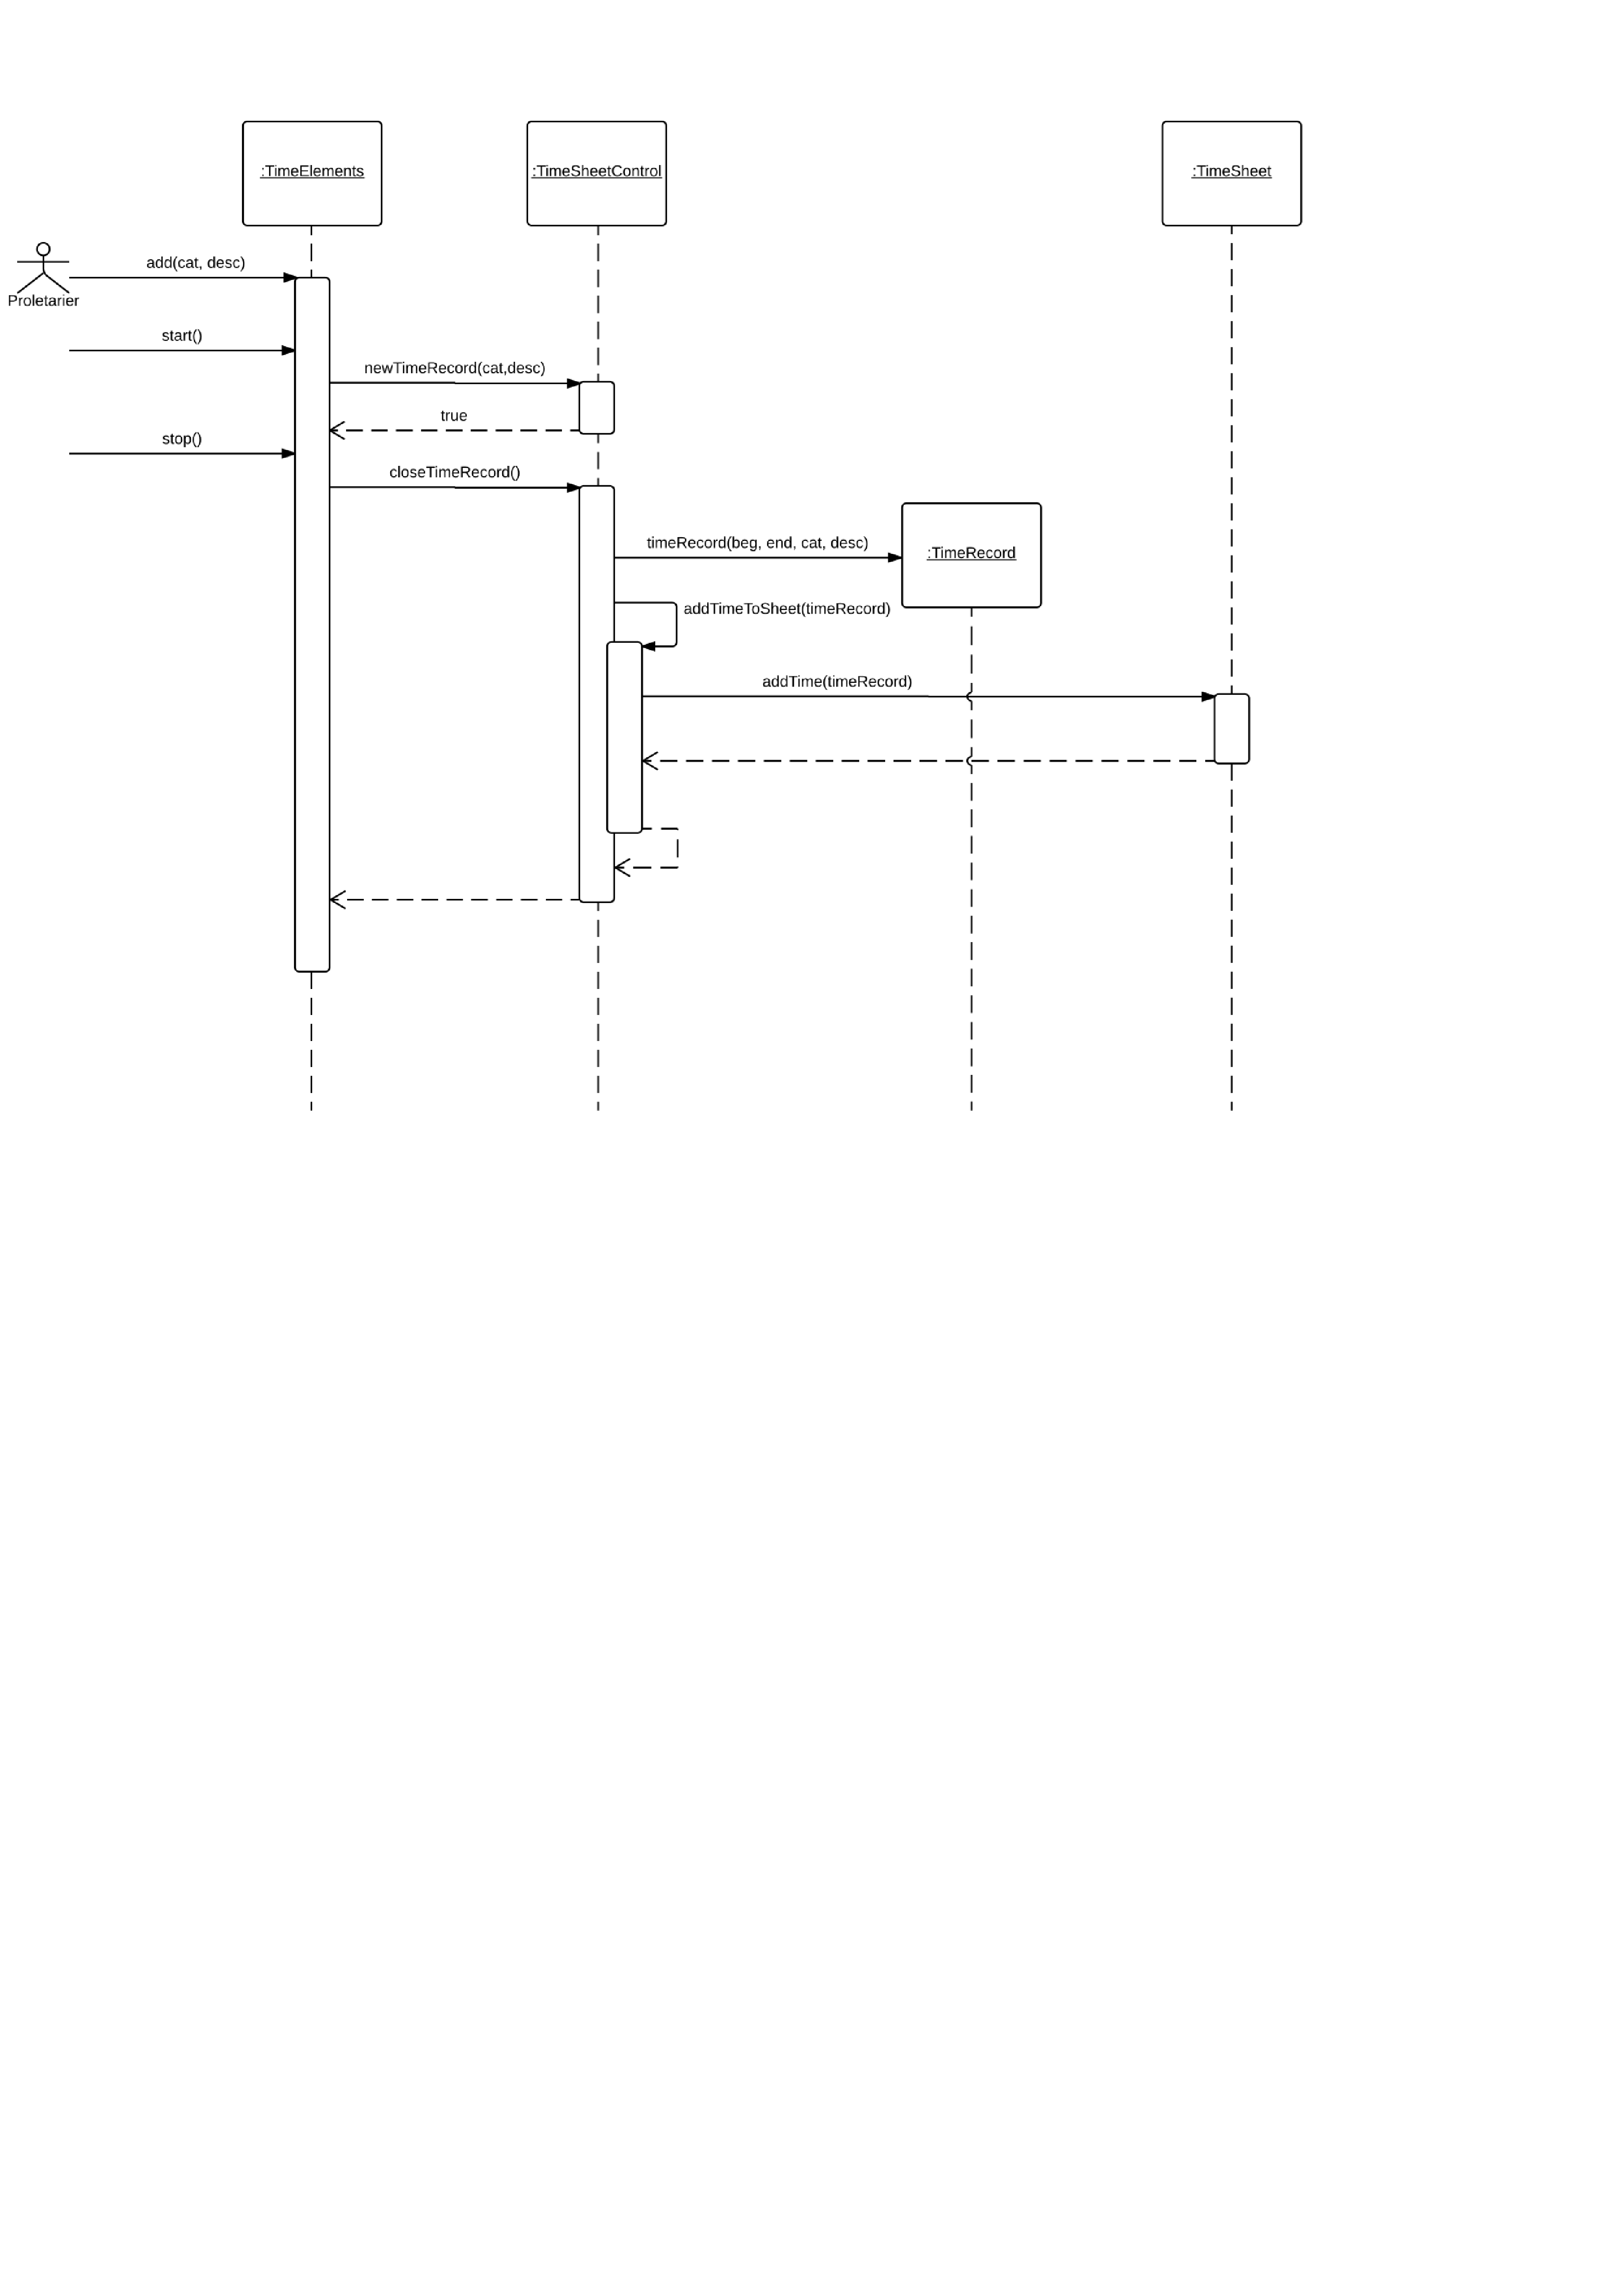
\includegraphics[width=\linewidth]{new-Time-record.pdf}
   \caption{Alte Zeiterfassungssequenz}
\end{figure}

\paragraph{Veränderungen}
\begin{itemize}
    \item Der Ablauf wurde in einklag mit Hibernate gebracht.
    \begin{itemize}
        \item Die TimeSheetControl kommuniziert nurnoch mit dem TimeSheetDAO
        \item TimeRecords werden erstellt und gespeichert, sobald die Zeiterfassung gestartet wurde(erhöhte persistenz)
        \item Wird der Tiem record geschlossen wird an dem jüngsten TimeRecord eine Endzeit hinzugefügt.
    \end{itemize}
    \item Das durchreichen von Wahrheitswerten wurde durch internes error handling ersetzt.
\end{itemize}

\begin{figure}
  \centering
    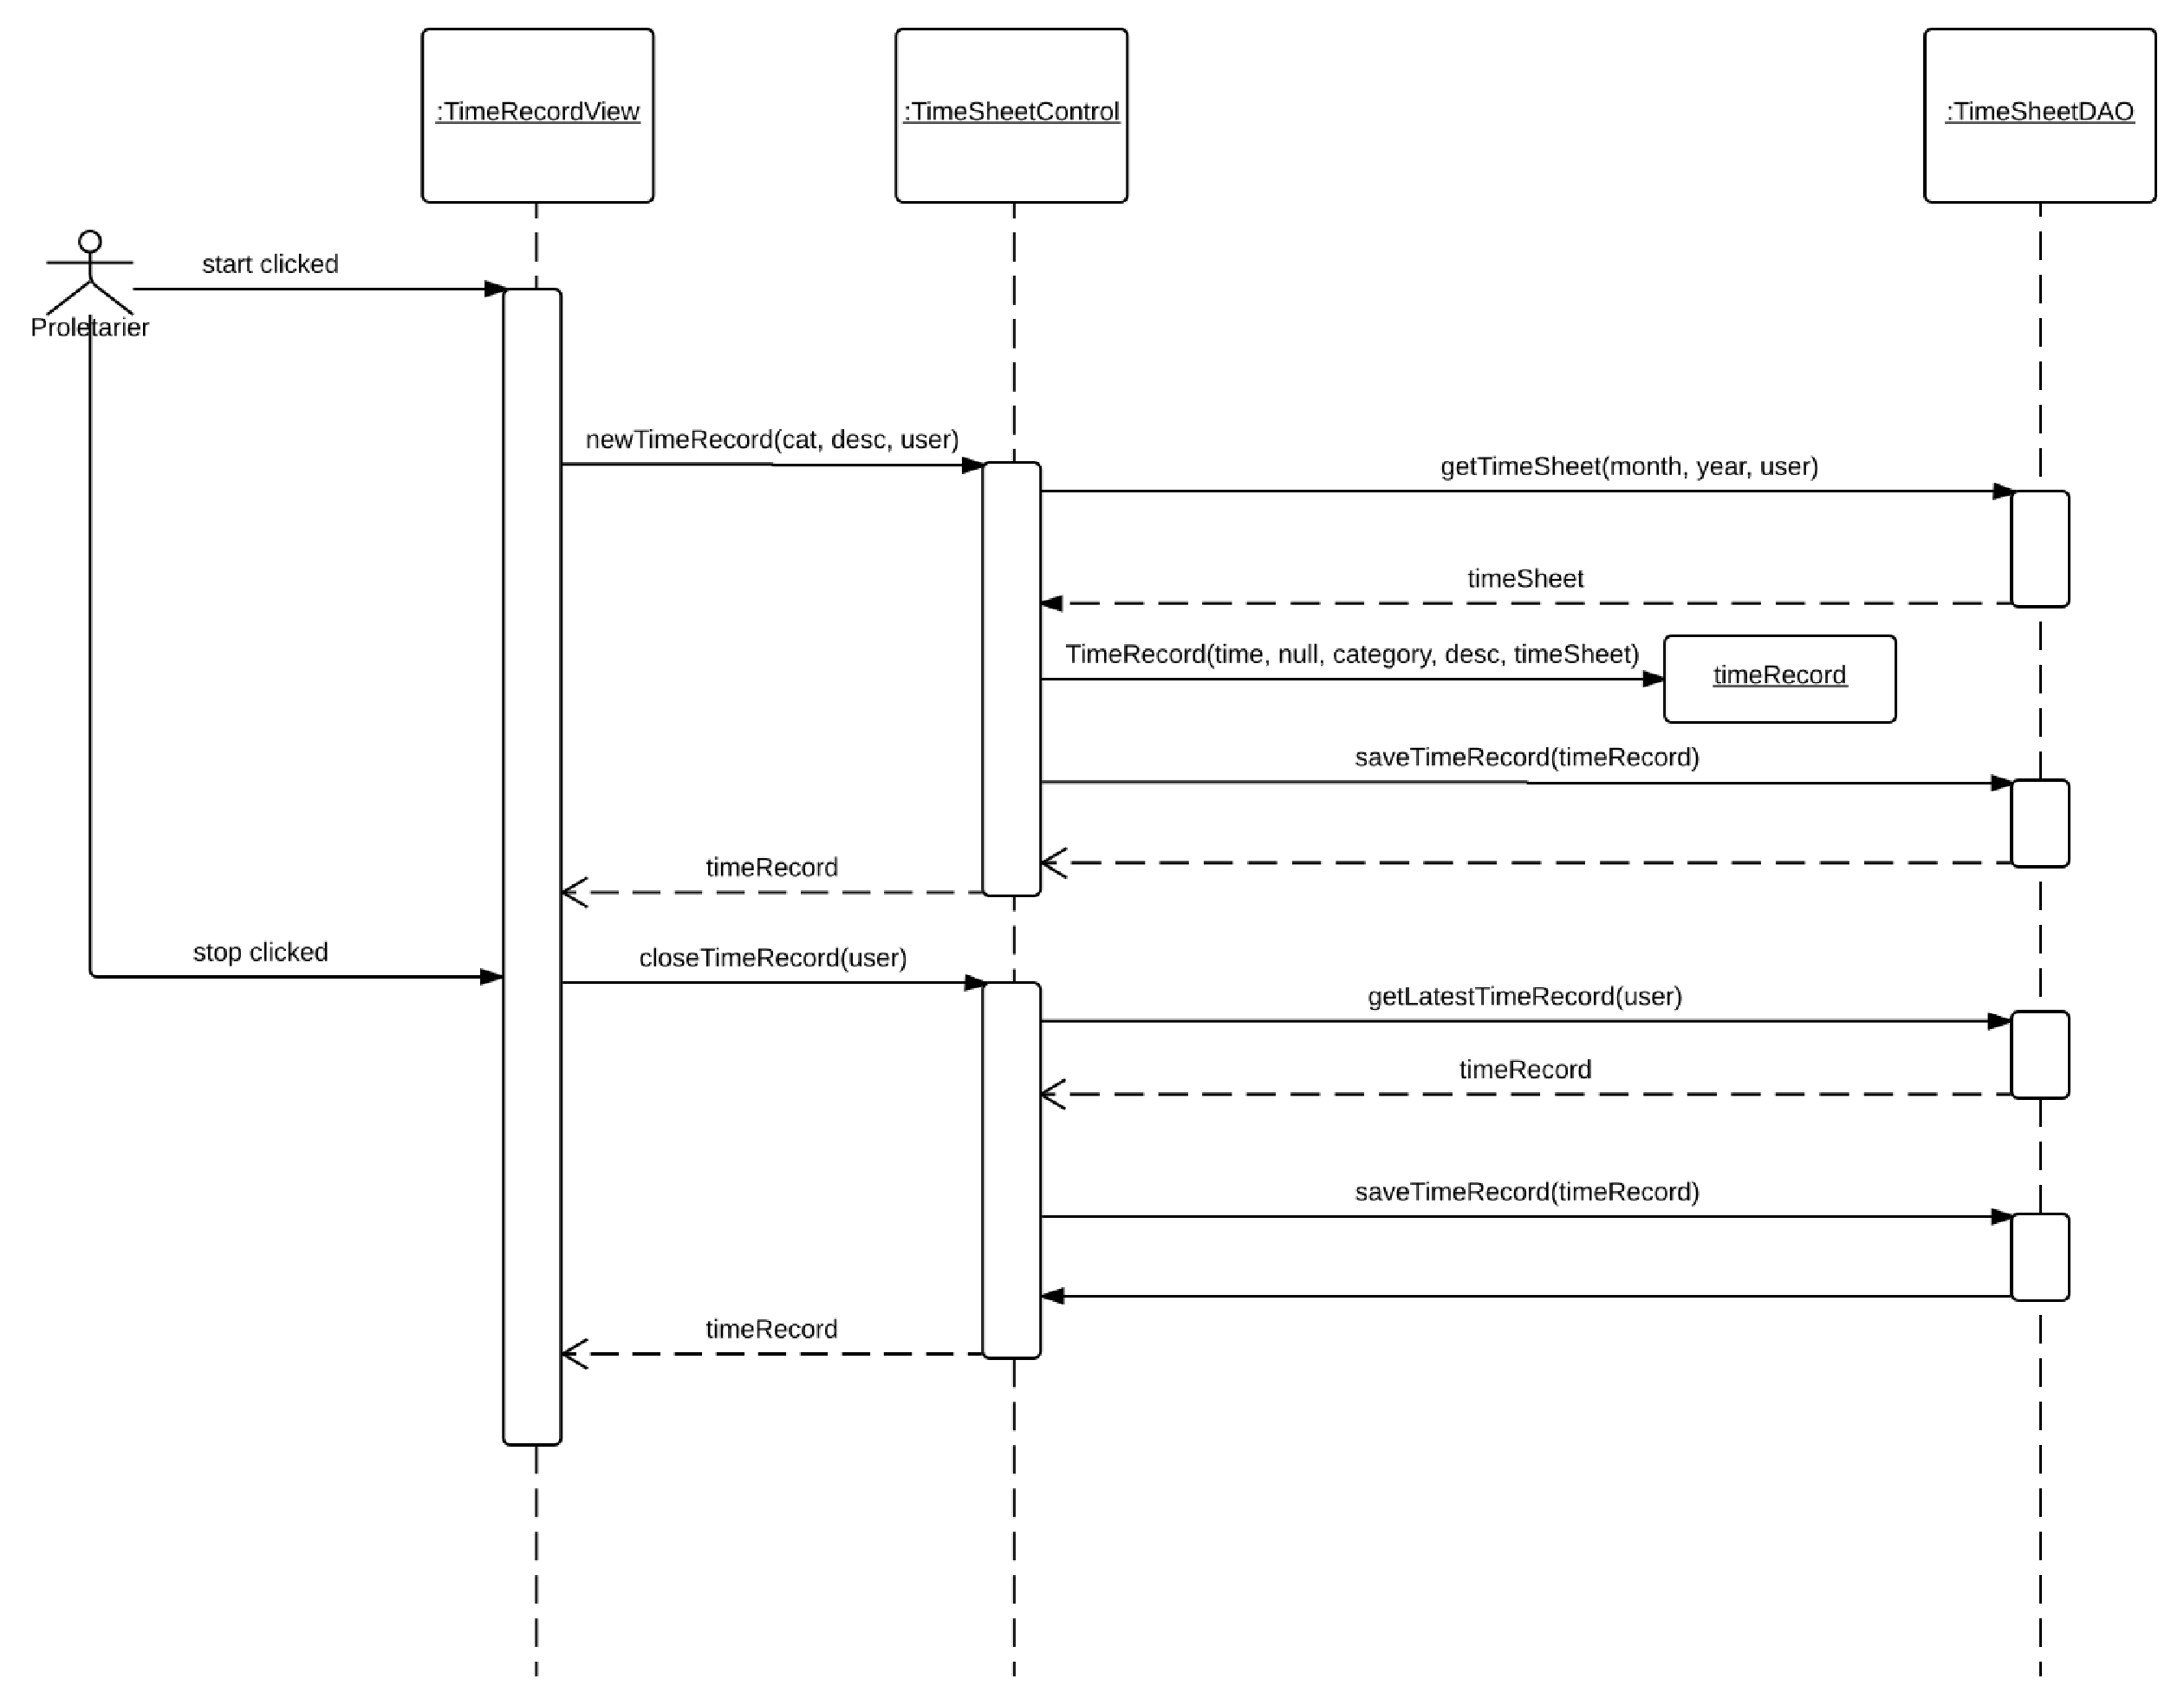
\includegraphics[width=\linewidth]{new-Time-record-new.pdf}
   \caption{Neue Zeiterfassungssequenz}
\end{figure}

\subsection{Admin druckt alle Stundenzettel - Sequenz}

\begin{figure}
  \centering
    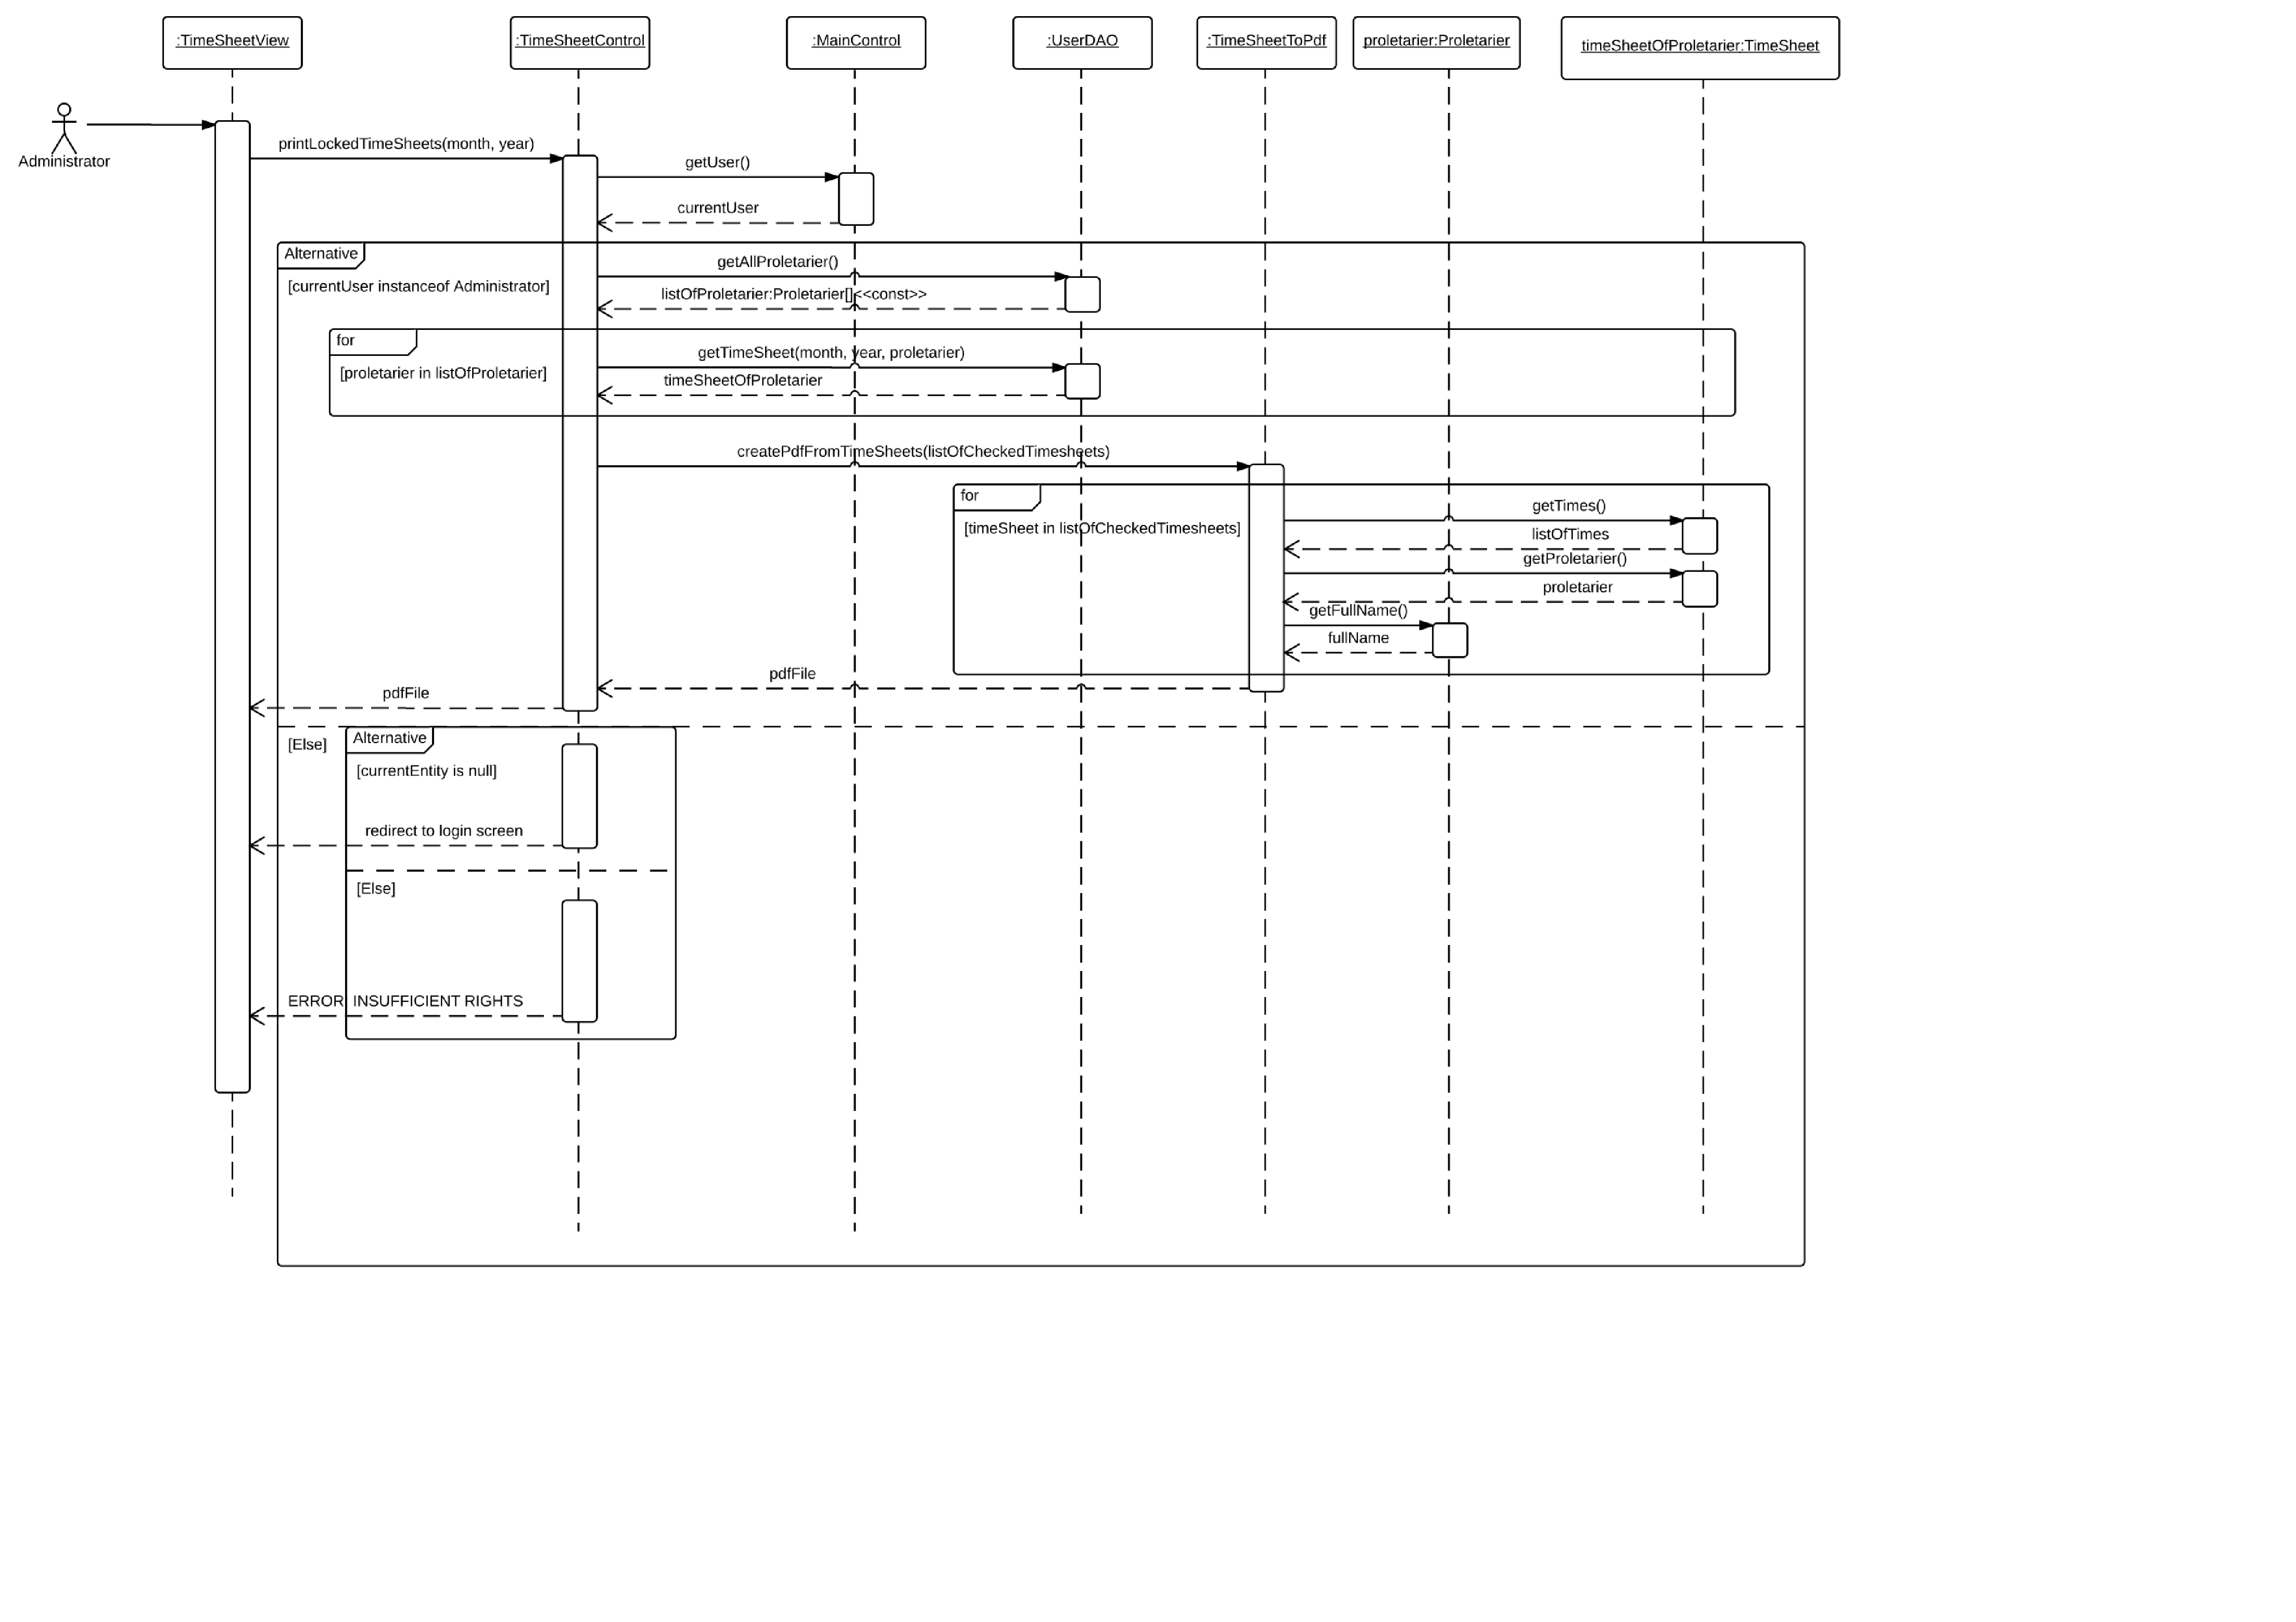
\includegraphics[width=\linewidth]{Admin-prints-all-timesheets.pdf}
   \caption{Alte Admin druckt Sequenz}
\end{figure}

\paragraph{Veränderungen}
\begin{itemize}
    \item Der Ablauf durch Hibernate stark vereinfacht
    \begin{itemize}
        \item Anstatt durch die for Schleifen die Stundezettel iterativ zu sammeln, genügt nun eine SQL abfrage im DAO um alle Stundenzettel zu erhalten
    \end{itemize}
    \item Das drucken übernimmt nun eine Subfunktion des TimeSheetHandlers
\end{itemize}

\begin{figure}
  \centering
    %\includegraphics[width=\linewidth]{}
   \caption{Aufgrund der Vereinfachungen durch hibernate ist ein Sequenzdiagramm hier nicht notwendig}
\end{figure}
